\documentclass[12pt,a4paper]{article}
\usepackage[MeX]{polski}
\usepackage[utf8]{inputenc}
\usepackage{tocloft}
\usepackage{amsmath}
\usepackage{graphicx}
\usepackage{caption}
\usepackage{subcaption}
\graphicspath{ {./images/} }
\usepackage{hyperref}
\hypersetup{
    colorlinks=true,
    linkcolor=blue,
    filecolor=magenta,      
    urlcolor=cyan,
    pdftitle={Overleaf Example},
    pdfpagemode=FullScreen,
    }

\urlstyle{same}
\renewcommand{\cftsecfont}{\normalfont\slshape}  
\renewcommand{\cftsubsecfont}{\normalfont\itshape}   
\renewcommand{\cftsubsubsecfont}{\normalfont\small} 

\title{\textit{Ciąg Fibonacciego}}
\author{Wiktor Czesnowski}

\begin{document}
\maketitle

\tableofcontents
\newpage
\section{\Large{Ciąg Fibonacciego w matematyce}}
W Matematyce \textbf{Liczby Fibonacciego} często oznaczone jako \textit{F\textsubscript{n}} tworzą ciąg o nazwie \textbf{Ciąg Fibonacciego} w którym każda kolejna liczba jest sumą dwóch pozostałych. Ciąg ten jest określony rekurencyjnie w sposób następujący: 
\[
	\textit{F\textsubscript{n}} =
\begin{cases}
	0 & \text{dla n = 0,}\\
	1 & \text{dla n = 1,}\\
	\textit{F\textsubscript{n-1}} + \textit{F\textsubscript{n-2}} & \text{dla n} > 0.
\end{cases}
\]
Pierwsze dziesięć wyrazów ciągu Fibonacciego to:
\begin{center}
\begin{tabular}{ |c| c| c| c| c| c| c| c| c| c|}
\hline 
\textit{F\textsubscript{0}} & \textit{F\textsubscript{1}} & \textit{F\textsubscript{2}} & \textit{F\textsubscript{3}} & \textit{F\textsubscript{4}} & \textit{F\textsubscript{5}} & \textit{F\textsubscript{6}} & \textit{F\textsubscript{7}} & \textit{F\textsubscript{8}} & \textit{F\textsubscript{9}} \\ 
\hline
0 & 1 & 1 & 2 & 3 & 5 & 8 & 13 & 21 & 34 \\
\hline
\end{tabular}
\end{center}
Ciąg został omówiony przez Leonarda z Pizy, zwannego Fibonaccim, w dziele Liber abaci jako rozwiązanie zadania o rozmnażaniu się królików. Nazwę "ciąg Fibonacciego" spopularyzował w XIX w. \'Edouard Lucas.%dodać odwołania!!
\subsection{\large{Podobne Ciągi}}
\subsubsection{Ciąg "Tribonacciego"}
Różni się od ciągu Fibonacciego tym, że każdy kolejny jego wyraz powstaje przez zsumowanie poprzednich trzech wyrazów zamiast dwóch.
Jego kilka początkowych wyrazów to: 0, 0, 1, 1, 2, 4, 7, 13, 24, 44, 81, 149, 274, 504, 927, 1705, 3136, 5768, 10609, 19513, 35890...\newline\newline
Stała "Tribonacciego" jest granicą ciągu: $\mathit{\frac{T(n + 1)}{T(n)}}$(gdzie \textbf{\textit{T}(n)} jest \textit{\textbf{n}}-tym wyrazem ciągu "Tribonacciego"), czyli analogiem złotej liczby dla ciągu Fibonacciego. Jest ona pierwiastkiem wielomianu \textit{ x\textsuperscript{3} - x\textsuperscript{2} - x -1 } oraz równania\newline 
\textit{x +  x\textsuperscript{-3}} =2 i wynosi ok. 1,83929.
\subsubsection{Ciąg "Tetranacciego"}
Różni się od ciągu Fibonacciego tym, każdy kolejny jego wyraz powstaje przez zsumowanie poprzednich czterech wyrazów zamiast dwóch
Jego kilka początkowych wyrazów to: 0, 0, 0, 1, 1, 2, 4, 8, 15, 29, 56, 108, 208, 401, 773, 1490, 2872, 5536, 10671, 20569...\newline\newline
Stała „Tetranacciego” jest granicą ciągu: $\mathit{\frac{T(n + 1)}{T(n)}}$(gdzie \textbf{\textit{T}(n)} jest \textit{\textbf{n}}-tym wyrazem ciągu "Tetranacciego").
Jest ona pierwiastkiem wielomianu \textit{x\textsuperscript{4} - x\textsuperscript{3} - x\textsuperscript{2} - x -1 } oraz równania \textit{x +  x\textsuperscript{-4}} = 2
i wynosi ok. 1,92756.
\newpage
\section{\Large{Ciąg Fibonacciego w innych dziedzinach}}
\subsection{\large{Ciąg Fibonacciego w biologii}} %dodać odwołania!
W kształtach wielu roślin widać linie spiralne. Na przykład na owocu ananasa 8 takich linii biegnie w jedną stronę, a 5 lub 13 w przeciwną. Na tarczy słonecznika może się krzyżować 55 spiral z 89 (liczby te bywają większe). Również różyczki kalafiora ułożone są spiralnie.

U większości roślin takie organy jak łodyga, liście czy kwiaty rozwijają się z małego, centralnie usytuowanego skupiska komórek – merystemu. Każdy zawiązek nowego organu (zwany primordium) wyrasta z merystemu w innym kierunku, pod pewnym kątem w stosunku do zawiązka, który pojawił się wcześniej. Okazuje się, że u wielu roślin ten kąt jest taki sam i że to właśnie dzięki niemu powstają wspomniane linie spiralne. Ten kąt to w przybliżeniu 137,5 stopnia (jest to tak zwany „Złoty kąt”). „Złotego kąta” nie da się wyrazić ułamkiem zwykłym. Jego dopełnienie do 360 stopni wynosi w przybliżeniu 5/8 kąta pełnego, dokładniej jest to 8/13 kąta pełnego, jeszcze dokładniej 13/21 i tak dalej (oparcie na liczbach \textbf{Fibonacciego}), ale żaden ułamek zwykły nie odpowiada mu ściśle.

Kiedy pojawiają się kolejne zawiązki, to jeśli każdy następny utworzy z poprzednim wspomniany „złoty kąt”, nigdy nie dojdzie do tego, by dwa z nich (lub więcej) rozwijały się w tym samym kierunku. Dzięki temu organy nie wyrastają z merystemu promieniście, lecz układają się w linie spiralne.
\newpage
\subsection{\large{Ciąg Fibonacciego w muzyce}}
Niektórzy muzykolodzy dopatrują się istnienia ciągu Fibonacciego w utworach muzycznych oraz w budowie instrumentów. Zależności takie występują w utworach muzycznych – najczęściej w proporcjach rytmicznych. Węgierski muzykolog Erno LendvaiInformacje powiązane z artykułem „Erno Lendvai” wykrył wiele takich zależności w muzyce Beli Bartóka, przede wszystkim w Muzyce na instrumenty strunowe, perkusję i czelestę, gdzie w części I kolejne odcinki formy zaczynają się w następującym porządku:
\begin{itemize}
\item zakończenie ekspozycji – t. 21,
\item początek stretto – t. 34,
\item kulminacja części – t. 55,
\item koniec części – t. 89.
\end{itemize}
W drugiej połowie XX wieku \textbf{ciąg Fibonacciego} stosowany był przez niektórych kompozytorów do proporcjonalnego porządkowania rytmu lub harmonii. Szczególnie często sięgali do niego kompozytorzy stosujący technikę serialną, np.: Karlheinz Stockhausen Klavierstück IX, Luigi Nono Il canto sospeso, Cristóbal Halffter Fibonacciana. Na \textbf{ciągu Fibonacciego} stosowanym równocześnie w przód i wstecz zbudowane jest Trio klarnetowe Krzysztofa Meyera. Jednostką miary jest w tym utworze ćwierćnuta, a kolejne odcinki różnią się obsadą, np.:
\begin{itemize}
\item kolejne odcinki grane przez fortepian mają długość: 89, 55, 34, 21, 13 ćwierćnut,
\item wszystkie instrumenty razem grają: 21, 34, 55, 89, 144 ćwierćnut.
\end{itemize}
\textbf{Ciąg Fibonacciego} używany jest też przez twórców spoza muzyki klasycznej, np. zespół Tool wykonujący muzykę z pogranicza rocka i metalu progresywnego w albumie Lateralus w tytułowym utworze użył \textbf{ciągu Fibonacciego} do stworzenia linii wokalnej.
\newpage
\subsection{\large{Ciąg Fibonacciego w literaturze}}
Motyw \textbf{ciągu Fibonacciego} wykorzystany został także w utworach literackich. W książce Kod Leonarda da Vinci Dana Browna stanowi on element jednego z kodów, który muszą złamać główni bohaterowie. W powieści Gniazdo światów Marka Huberatha \textbf{ciąg Fibonacciego} jest podstawą struktury wszechświata, na której oparte są kolejne jego poziomy.

Istnieją też utwory poetyckie nawiązujące formą do ciągu Fibonacciego. Współczesny poeta polski Marcin Orliński (na potrzeby czasopisma satyrycznego) nazwał ten gatunek fibonagramem. W obrębie fibonagramu wyróżnił fibonagram literowy (liczba liter w kolejnych wyrazach odpowiada wartości kolejnych wyrazów w ciągu) i fibonagram wyrazowy (liczba słów w wersie odpowiada wartości kolejnych wyrazów w ciągu).
\subsection{\large{Ciąg Fibonacciego w sztuce}}
Złoty podział jest granicą stosunków kolejnych wyrazów \textbf{ciągu Fibonacciego} (a także każdego ciągu opartego na podobnych zasadach).
\begin{figure}[h]
\begin{subfigure}{.5\textwidth}
\centering
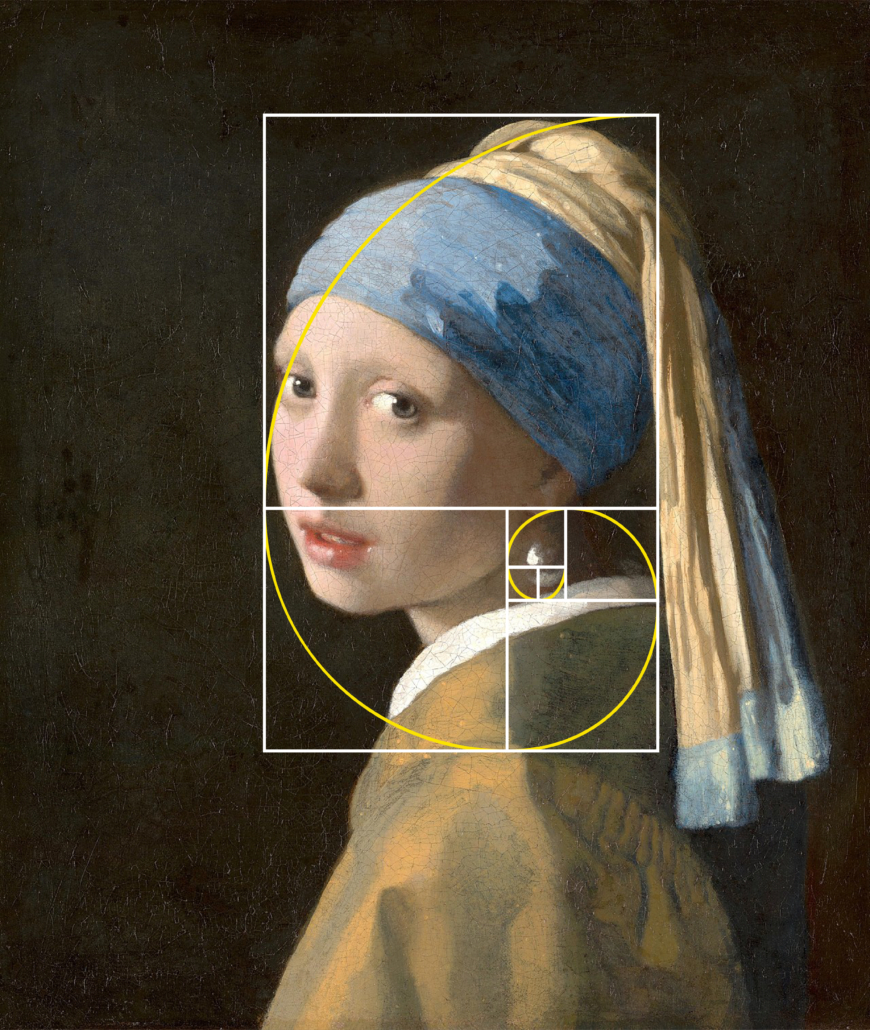
\includegraphics[width=0.5\textwidth]{girlpearl}
\caption{Vermeer, Girl with a Pearl Earring.}
\label{Vermeer, Girl with a Pearl Earring.}
\end{subfigure}
\begin{subfigure}{.5\textwidth}
\centering
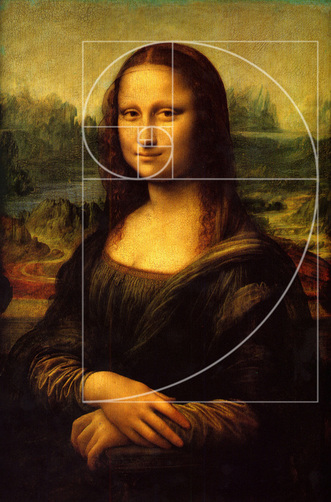
\includegraphics[width=0.4\textwidth]{monalisa}
\caption{Leonardo da Vinci, Mona Lisa.}
\label{Leonardo da Vinci, Mona Lisa.}
\end{subfigure}
\end{figure}
\end{document}